% This Latex poster uses the baposter class, originally from
% http://www.brian-amberg.de/uni/poster. Versions are found in several places.
% The files on which this version is based are from circulation within WASP
% and exact origins are not known.
%
% CONTENT
% To update the poster, modify the contents in the parts/ folder.
% The file header.tex contains convenience commands such as \title, \companylogo etc.
% Other files contain pure formatting.
%
% COLORS
% The following standard colors are defined: wasp_text, wasppink, waspgrey, waspblue
%
% Enjoy!
% Per Skarin, 2021

\documentclass[a0paper,portrait]{baposter}
\usepackage{lipsum}  
\usepackage{relsize}	% For \smaller
\usepackage{url}	% For \url
\usepackage{epstopdf}	% Included EPS files automatically converted to PDF to include with pdflatex
\usepackage[utf8]{inputenc} 
\usepackage{multirow}
\usepackage{booktabs}
\usepackage[labelfont=bf]{caption}
\usepackage{enumitem}
\usepackage{tcolorbox}
\usepackage{mathtools}

% PATHS
\graphicspath{{template-images/}{content-images/}}

% FONTS AND COLORS
\renewcommand{\familydefault}{\sfdefault}
\newcommand{\mytitlefont}{\fontfamily{\familydefault}\selectfont }
\newcommand{\mytextfont}{\fontfamily{\familydefault}\selectfont }
% Comment the four lines below to skip WASP fonts
\usepackage{MinionPro}
\usepackage{MyriadPro}
\renewcommand{\mytitlefont}{\fontfamily{MyriadPro-LF}\selectfont }
\renewcommand{\mytextfont}{\fontfamily{MinionPro-LF}\selectfont }

\definecolor{wasppink}{RGB}{203,166,169} 
\definecolor{waspgrey}{RGB}{88,89,91}
\definecolor{waspblue}{RGB}{26,141,173}
\definecolor{darkgreen}{rgb}{0,0.6,0}

\definecolor{wasp_text}{RGB}{66,80,82}
\colorlet{wasp_banner_light}{waspblue}
\colorlet{wasp_banner_dark}{waspgrey}

% LIST SETTINGS
\setlist{itemsep=.1em, leftmargin=1em}

% COMMANDS
\newcommand\thetitle{}\renewcommand\title[1]{\renewcommand\thetitle{#1}}
\newcommand\theauthor{}\renewcommand\author[1]{\renewcommand\theauthor{#1}}
\newcommand\thedepinfo{}\newcommand\depinfo[1]{\renewcommand\thedepinfo{#1}}
\newcommand\thesupervisors{}\newcommand\supervisors[1]{\renewcommand\thesupervisors{#1}}
\newcommand\theuniversitylogo{}\newcommand\universitylogo[1]{\renewcommand\theuniversitylogo{#1}}
\newcommand\thecompanylogo{}\newcommand\companylogo[1]{\renewcommand\thecompanylogo{#1}}


%%%%%%%%%%%%%%%%%%%%%%%%%%%%%%%%%%%%%%%%%%%%%%%%%%%%%%%%%%%%%%%%%%%%%%%%%%%%%%%
%%% Document Start %%%%%%%%%%%%%%%%%%%%%%%%%%%%%%%%%%%%%%%%%%%%%%%%%%%%%%%%%%%%
%%%%%%%%%%%%%%%%%%%%%%%%%%%%%%%%%%%%%%%%%%%%%%%%%%%%%%%%%%%%%%%%%%%%%%%%%%%%%%%

% Text to the left
\title{Specific research and break-throughs}
\author{John Doe, Ind. PhD, Company and Lund University}
\depinfo{Dept. of Automatic Control, A Project Within This Department}
\supervisors{Prof. Calculus (LU), Dr. Gadget (Company) and Another Person (LU)}

% Logos on the right. Put the images in template-images/
\universitylogo{
\includegraphics[width=0.7\textwidth]{university/lund}}
\companylogo{
\includegraphics[width=0.6\textwidth]{company/ericsson}}



\begin{document}

%%% General Poster Settings %%%%%%%%%%%%%%%%%%%%%%%%%%%%%%%%%%%%%%%%%%%%%%%%%%%
%%%%%% Eye Catcher, Title, Authors and University Images %%%%%%%%%%%%%%%%%%%%%%
\begin{poster}{
 % Show grid to help with alignment
 grid=false,
 % eyecatcher=false,
 % Column spacing
 colspacing=1em,
 columns=2,
 boxpadding=.5cm,
 % Color style
 headerColorOne=wasp_banner_light,
 borderColor=wasp_banner_light,
 headerFontColor=cyan!10!white,
 % Format of textbox
 textborder=faded,
 % Format of text header
 headerborder=open,
 headershape=roundedright,
 headershade=plain,
 background=none,
 % bgColorOne=cyan!10!white,
 headerheight=0.12\textheight}
%%% Eye Cacther %%%%%%%%%%%%%%%%%%%%%%%%%%%%%%%%%%%%%%%%%%%%%%%%%%%%%%%%%%%%%%%
{
	Eye Catcher, empty if option eyecatcher=false - unused
}
%%%% Title %%%%%%%%%%%%%%%%%%%%%%%%%%%%%%%%%%%%%%%%%%%%%%%%%%%%%%%%%%%%%%%%%%%%%
{
	\textcolor{wasp_text}{\mytitlefont \huge \thetitle}
}
%%% Authors %%%%%%%%%%%%%%%%%%%%%%%%%%%%%%%%%%%%%%%%%%%%%%%%%%%%%%%%%%%%%%%%%%%
{
  \vspace{0.5em}
  \textcolor{wasp_text}{\Large \theauthor\\
	\large \thedepinfo\\
	Supervisors: \thesupervisors\\
	}
}
%%% Logo %%%%%%%%%%%%%%%%%%%%%%%%%%%%%%%%%%%%%%%%%%%%%%%%%%%%%%%%%%%%%%%%%%%%%%
{
  \begin{minipage}{8cm}
   \centering
   \vspace{0.5cm}
	    \theuniversitylogo\vspace{0.25cm}\par
		  \thecompanylogo
  \end{minipage}
}

%%%%%%%%%%%%%%%%%%%%%%%%%%%%%%%%%%%%%%%%%%%%%%%%%%%%%%%%%%%%%%%%%%%%%%%%%%%%%%
%%% Now define the boxes that make up the poster
%%%---------------------------------------------------------------------------
%%% Each box has a name and can be placed absolutely or relatively.
%%% The only inconvenience is that you can only specify a relative position 
%%% towards an already declared box. So if you have a box attached to the 
%%% bottom, one to the top and a third one which should be inbetween, you 
%%% have to specify the top and bottom boxes before you specify the middle 
%%% box.
%%%%%%%%%%%%%%%%%%%%%%%%%%%%%%%%%%%%%%%%%%%%%%%%%%%%%%%%%%%%%%%%%%%%%%%%%%%%%%

%%%%%%%%%%%%%%%%%%%%%%%%%%%%%%%%%%%%%%%%%%%%%%%%%%%%%%%%%%%%%%%%%%%%%%%%%%%%%%
  \headerbox{\mytitlefont Motivation \& Research Goals}{name=description,column=0,row=0,span=2}{
  \mytextfont
%%%%%%%%%%%%%%%%%%%%%%%%%%%%%%%%%%%%%%%%%%%%%%%%%%%%%%%%%%%%%%%%%%%%%%%%%%%%%%
  % Put the motivation behind and goals of the research here
\large
\lipsum[2]

}

%%%%%%%%%%%%%%%%%%%%%%%%%%%%%%%%%%%%%%%%%%%%%%%%%%%%%%%%%%%%%%%%%%%%%%%%%%%%%%
  \headerbox{\mytitlefont Methods}{name=motivation,column=0,row=0,span=1, below=description}{
%%%%%%%%%%%%%%%%%%%%%%%%%%%%%%%%%%%%%%%%%%%%%%%%%%%%%%%%%%%%%%%%%%%%%%%%%%%%%%
  \mytextfont
  % The methods that you use goes here
\vspace{0.3cm}
\begin{center}
  \vspace{-0.4cm}
  
\includegraphics[width=.9\linewidth]{homer_equation}
\end{center}
\vspace{0.25em}
\textsuperscript{[1]}\lipsum[1]
\begin{alignat*}{2}
  u^*(x) := argmin\quad &\mathrlap{\sum_{i=0}^{N-1} l(x_i, u_i) + V_f(X_{N})}&&\\
  \text{subject to}\quad &x_{i+1} &&=\quad f(x_i, u_i),\\
  &g(x_i, u_i)\quad && \le\quad 0\\
  &x_0 &&=\quad x,\\
  &x_N &&\in\quad \mathcal{T}
\end{alignat*}
Lorem ipsum dolor sit amet, consectetuer adipiscing elit. Aenean commodo ligula eget dolor. Aenean massa. Cum sociis natoque penatibus et magnis dis parturient montes, nascetur ridiculus mus. Donec quam felis, ultricies nec, pellentesque eu, pretium quis, sem.
\vspace{2em} % Fill in to put references at the bottom

}

%%%%%%%%%%%%%%%%%%%%%%%%%%%%%%%%%%%%%%%%%%%%%%%%%%%%%%%%%%%%%%%%%%%%%%%%%%%%%%
  \headerbox{\mytitlefont Selected Results}{name=goal,column=1,row=0,span=1, below=description }{
%%%%%%%%%%%%%%%%%%%%%%%%%%%%%%%%%%%%%%%%%%%%%%%%%%%%%%%%%%%%%%%%%%%%%%%%%%%%%%
  \mytextfont
  % Put some results here
	 \textsuperscript{[2]}\lipsum[4]\par
  	\begin{center}
	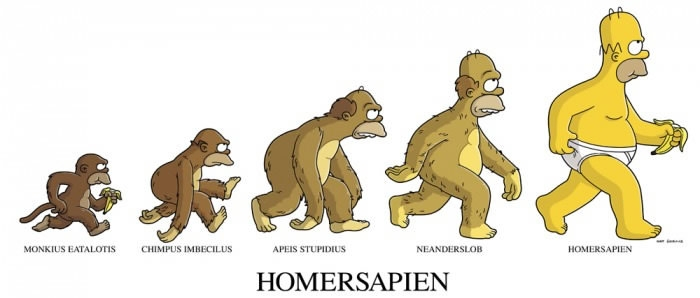
\includegraphics[width=.9\linewidth]{homersapien}
	\end{center}	
	\begin{tcolorbox}
	\lipsum[66]
	\end{tcolorbox}
\par
\vspace{1.5em}
\lipsum[75]
\vspace{1.5em}
\par
\begin{tikzpicture}
	\node[anchor=west] at (0,0) {
		\begin{minipage}{0.2\textwidth}
		\centering
		\resizebox{\textwidth}{!}{
\includegraphics{homer_smart}}
		\end{minipage}
	};
	\node[anchor=east] at (\textwidth,0) {
		\begin{minipage}{0.7\textwidth}
		\begin{tcolorbox}
Lorem ipsum dolor sit amet, consectetuer adipiscing elit. Aenean commodo ligula eget dolor. Aenean massa. Cum sociis natoque penatibus et magnis dis parturient montes, nascetur ridiculus mus. Donec quam felis, ultricies nec, pellentesque eu, pretium quis, sem. \textsuperscript{[3]}.
		\end{tcolorbox}
		\end{minipage}
	};
\end{tikzpicture}
\vspace{1.5em}
\begin{tcolorbox}
	\lipsum[66]
\end{tcolorbox}


}

%%%%%%%%%%%%%%%%%%%%%%%%%%%%%%%%%%%%%%%%%%%%%%%%%%%%%%%%%%%%%%%%%%%%%%%%%%%%%%
  \headerbox{References}{headerColorOne=wasp_banner_dark, borderColor=wasp_banner_dark, name=results,column=0,row=0,span=1, below=motivation }{
%%%%%%%%%%%%%%%%%%%%%%%%%%%%%%%%%%%%%%%%%%%%%%%%%%%%%%%%%%%%%%%%%%%%%%%%%%%%%%
	\mytextfont
  \small
\vspace{-0.5cm}
\fcolorbox{white}{white}{\hspace{-0.5cm}\parbox{0.1\linewidth}{\centering [1]}\parbox{1.3cm}{
\includegraphics[trim=28mm 10mm 35mm 15mm,clip,width=0.8cm]{qracm}}\parbox{0.7\linewidth}{\footnotesize\smaller Five Challenges in Cloud-Enabled Intelligence and Control\\\tiny T. Abdelzaher, Y. Hao, K. Jayarajah, A. Misra, S. Yao, P. Skarin, D. Weerakoon and K. {\AA}rz{\'e}n\\ACM Transactions on Internet Technology, 2019}}\par\vspace{-0.4cm}
	
\fcolorbox{white}{white}{\hspace{-0.5cm}\parbox{0.1\linewidth}{\centering [2]}\parbox{1.3cm}{
\includegraphics[trim=25mm 10mm 35mm 10mm,clip,width=0.8cm]{qredge1}}\parbox{0.7\linewidth}{\footnotesize\smaller Towards Mission-Critical Control at the Edge and Over 5G\\\tiny Per Skarin, William Tärneberg, Karl-Erik Årzén, Maria Kihl\\Best paper award, IEEE Services (EDGE), 2-7 July, 2018, San Fran., CA, USA}}\par\vspace{-0.25cm}
	
\fcolorbox{white}{white}{\hspace{-0.5cm}\parbox{0.1\linewidth}{\centering [5]}\parbox{1.3cm}{
\includegraphics[trim=28mm 35mm 35mm 35mm,clip,width=0.8cm]{qrifac}}\parbox{0.7\linewidth}{\footnotesize\smaller Cloud-based model predictive control with variable horizon\\\tiny Per Skarin, Johan Eker, Karl-Erik Årzén\\Subm. to 21st World Congress of the International Federation of Automatic Control, 2020}}\par\vspace{-0.3cm}

}

\headerbox{}{name=foottext, column=0, span=2, above=bottom, textborder=none,headerborder=none,boxheaderheight=0pt,boxColorOne=wasp_banner_dark}{\hfill 
\includegraphics[height=1cm]{waspwhite}}


\end{poster}
\end{document}
